% !TeX document-id = {a7325568-63cb-46d1-95d6-777a45054e5a}
% !TeX TXS-program:compile = txs:///pdflatex/[--shell-escape]
\documentclass{article}
\usepackage{style}
\begin{document}
\maketitle
\tableofcontents
\section{Introducción}
Un perceptrón multicapa es tipo de red neuronal artifical compuesta de varias neuronas y varias capas, puede resolver problemas que un perceptrón simple puede. El clásico ejemplo es el de la compuerta XOR:
\begin{figure}[h!]
	\caption{Compuerta XOR}
	\centering
	\includegraphics{xor}
\end{figure}
\\
En este caso se necesitan dos fronteras de desición, por ende dos neuron y se necesita otra capa para ``combinar los resultados''. La manera la cual se actualizan los pesos y bías del MLP es usando un algoritmo para propagar los resultados a las neuronas de la capa actual y de las anteriores, es algoritmo es llamado backpropagation, el cual es un algoritmo de minización basado en el descenso en gradiente el cual encuentra los mínimos locales de una función. En esta práctica se usan MLP's para aproximar señales leyendo datos de archivos de texto.
\newpage
\subsection{Modelo}
\begin{figure}[h!]
	\caption{Modelo}
	\centering
	\includegraphics[scale=1]{mlp}
\end{figure}
\subsubsection{Foward Propagation}
$$ a^0 = p$$
$$ a^{m+1} = f^{m+1}(W^{m+1} \cdot a^m + b^{m+1}), \text{m}=0,1,2,3,\dots,M-1$$
$$ a=a^M $$
donde $M$ es el número de capas.\\
\subsubsection{Foward Propagation}
Para poder usar backpropagation se necesita que las funciones de activación en cada capa sean continuas y derivables.
El algoritmo es el siguiente:
\begin{enumerate}
	\item Calcular las sensitividades de cada capa desde la última capa hasta la primera: 
	$$ s^M = -2\dot{F}^M(n^M)(t-a)$$
	$$ s^m = \dot{F}^m(n^m)(W^{m + 1})^T s^{m+1} $$
	\item Actualizar los pesos y bias:
	$$ w^{m}(k+1) = W^m(k)-\alpha s^m(a^m-1)^T $$
	$$ b^{m}(k+1) = b^m(k)-\alpha s^m $$	
\end{enumerate}

\newpage
\section{Diagrama de Flujo}
\begin{figure}[htpb]
	\centering
	\includesvg[width = 400pt, height = 400pt]{diagram}
	\caption{Diagrama de Flujo}
\end{figure}
\newpage
\section{Resultados}
\subsection{Polinomio 1}
\subsection{Inputs}
\begin{multicols}{4}
	\begin{enumerate}
		\item -2.0000
		\item -1.9600
		\item -1.9200
		\item -1.8800
		\item -1.8400
		\item -1.8000
		\item -1.7600
		\item -1.7200
		\item -1.6800
		\item -1.6400
		\item -1.6000
		\item -1.5600
		\item -1.5200
		\item -1.4800
		\item -1.4400
		\item -1.4000
		\item -1.3600
		\item -1.3200
		\item -1.2800
		\item -1.2400
		\item -1.2000
		\item -1.1600
		\item -1.1200
		\item -1.0800
		\item -1.0400
		\item -1.0000
		\item -0.9600
		\item -0.9200
		\item -0.8800
		\item -0.8400
		\item -0.8000
		\item -0.7600
		\item -0.7200
		\item -0.6800
		\item -0.6400
		\item -0.6000
		\item -0.5600
		\item -0.5200
		\item -0.4800
		\item -0.4400
		\item -0.4000
		\item -0.3600
		\item -0.3200
		\item -0.2800
		\item -0.2400
		\item -0.2000
		\item -0.1600
		\item -0.1200
		\item -0.0800
		\item -0.0400
		\item  0
		\item  0.0400
		\item  0.0800
		\item  0.1200
		\item  0.1600
		\item  0.2000
		\item  0.2400
		\item  0.2800
		\item  0.3200
		\item  0.3600
		\item  0.4000
		\item  0.4400
		\item  0.4800
		\item  0.5200
		\item  0.5600
		\item  0.6000
		\item  0.6400
		\item  0.6800
		\item  0.7200
		\item  0.7600
		\item  0.8000
		\item  0.8400
		\item  0.8800
		\item  0.9200
		\item  0.9600
		\item  1.0000
		\item  1.0400
		\item  1.0800
		\item  1.1200
		\item  1.1600
		\item  1.2000
		\item  1.2400
		\item  1.2800
		\item  1.3200
		\item  1.3600
		\item  1.4000
		\item  1.4400
		\item  1.4800
		\item  1.5200
		\item  1.5600
		\item  1.6000
		\item  1.6400
		\item  1.6800
		\item  1.7200
		\item  1.7600
		\item  1.8000
		\item  1.8400
		\item  1.8800
		\item  1.9200
		\item  1.9600
		\item  2.0000
	\end{enumerate}
\end{multicols}
\subsection{Targets}
\begin{multicols}{4}
\begin{enumerate}
	\item 1.0000 
	\item 1.2487 
	\item 1.4818 
	\item 1.6845 
	\item 1.8443 
	\item 1.9511 
	\item 1.9980 
	\item 1.9823 
	\item 1.9048 
	\item 1.7705 
	\item 1.5878 
	\item 1.3681 
	\item 1.1253 
	\item 0.8747 
	\item 0.6319 
	\item 0.4122 
	\item 0.2295 
	\item 0.0952 
	\item 0.0177 
	\item 0.0020 
	\item 0.0489 
	\item 0.1557 
	\item 0.3155 
	\item 0.5182 
	\item 0.7513 
	\item 1.0000 
	\item 1.2487 
	\item 1.4818 
	\item 1.6845 
	\item 1.8443 
	\item 1.9511 
	\item 1.9980 
	\item 1.9823 
	\item 1.9048 
	\item 1.7705 
	\item 1.5878 
	\item 1.3681 
	\item 1.1253 
	\item 0.8747 
	\item 0.6319 
	\item 0.4122 
	\item 0.2295 
	\item 0.0952 
	\item 0.0177 
	\item 0.0020 
	\item 0.0489 
	\item 0.1557 
	\item 0.3155 
	\item 0.5182 
	\item 0.7513 
	\item 1.0000 
	\item 1.2487 
	\item 1.4818 
	\item 1.6845 
	\item 1.8443 
	\item 1.9511 
	\item 1.9980 
	\item 1.9823 
	\item 1.9048 
	\item 1.7705 
	\item 1.5878 
	\item 1.3681 
	\item 1.1253 
	\item 0.8747 
	\item 0.6319 
	\item 0.4122 
	\item 0.2295 
	\item 0.0952 
	\item 0.0177 
	\item 0.0020 
	\item 0.0489 
	\item 0.1557 
	\item 0.3155 
	\item 0.5182 
	\item 0.7513 
	\item 1.0000 
	\item 1.2487 
	\item 1.4818 
	\item 1.6845 
	\item 1.8443 
	\item 1.9511 
	\item 1.9980 
	\item 1.9823 
	\item 1.9048 
	\item 1.7705 
	\item 1.5878 
	\item 1.3681 
	\item 1.1253 
	\item 0.8747 
	\item 0.6319 
	\item 0.4122 
	\item 0.2295 
	\item 0.0952 
	\item 0.0177 
	\item 0.0020 
	\item 0.0489 
	\item 0.1557 
	\item 0.3155 
	\item 0.5182 
	\item 0.7513 
	\item 1.0000
\end{enumerate}
\end{multicols}
\subsubsection{Datos}
\[V1=
\begin{bmatrix}
11 16 10 1
\end{bmatrix}\]

\[V2=
\begin{bmatrix}
3 2 1
\end{bmatrix}\]
epochmax = 10000\\
Múltiplo para las épocas de validación = 500\\
numval = 7\\
alpha=.0701\\
error de validación = .0000000000000001\\
Configuración: 80-15-15
\subsection{Resultado}
\subsection{Imágenes}
\begin{figure}[htpb]
	\centering
	\includesvg[width = 500pt, height = 500pt]{pol1/1}
	\caption{Gráfica 1.1}
\end{figure}

\begin{figure}[htpb]
	\centering
	\includesvg[width = 500pt, height = 500pt]{pol1/2}
	\caption{Gráfica 1.2}
\end{figure}

\begin{figure}[htpb]
	\centering
	\includesvg[width = 500pt, height = 500pt]{pol1/3}
	\caption{Gráfica 1.3}
\end{figure}

\begin{figure}[htpb]
	\centering
	\includesvg[width = 500pt, height = 500pt]{pol1/4}
	\caption{Gráfica 1.4}
\end{figure}

\begin{figure}[htpb]
	\centering
	\includesvg[width = 500pt, height = 500pt]{pol1/5}
	\caption{Gráfica 1.5}
\end{figure}

\begin{figure}[htpb]
	\centering
	\includesvg[width = 500pt, height = 500pt]{pol1/6}
	\caption{Gráfica 1.6}
\end{figure}

\begin{figure}[htpb]
	\centering
	\includesvg[width = 500pt, height = 500pt]{pol1/7}
	\caption{Gráfica 1.7}
\end{figure}

\begin{figure}[htpb]
	\centering
	\includesvg[width = 500pt, height = 500pt]{pol1/8}
	\caption{Gráfica 1.8}
\end{figure}

\begin{figure}[htpb]
	\centering
	\includesvg[width = 500pt, height = 500pt]{pol1/9}
	\caption{Gráfica 1.9}
\end{figure}
\newpage
\subsection{Polinomio 2}
\subsection{Inputs}
\begin{multicols}{4}
	\begin{enumerate}
		\item 4.0000
		\item 3.9667
		\item 3.9333
		\item 3.9000
		\item 3.8667
		\item 3.8333
		\item 3.8000
		\item 3.7667
		\item 3.7333
		\item 3.7000
		\item 3.6667
		\item 3.6333
		\item 3.6000
		\item 3.5667
		\item 3.5333
		\item 3.5000
		\item 3.4667
		\item 3.4333
		\item 3.4000
		\item 3.3667
		\item 3.3333
		\item 3.3000
		\item 3.2667
		\item 3.2333
		\item 3.2000
		\item 3.1667
		\item 3.1333
		\item 3.1000
		\item 3.0667
		\item 3.0333
		\item 3.0000
		\item 2.9667
		\item 2.9333
		\item 2.9000
		\item 2.8667
		\item 2.8333
		\item 2.8000
		\item 2.7667
		\item 2.7333
		\item 2.7000
		\item 2.6667
		\item 2.6333
		\item 2.6000
		\item 2.5667
		\item 2.5333
		\item 2.5000
		\item 2.4667
		\item 2.4333
		\item 2.4000
		\item 2.3667
		\item 2.3333
		\item 2.3000
		\item 2.2667
		\item 2.2333
		\item 2.2000
		\item 2.1667
		\item 2.1333
		\item 2.1000
		\item 2.0667
		\item 2.0333
		\item 2.0000
		\item 1.9667
		\item 1.9333
		\item 1.9000
		\item 1.8667
		\item 1.8333
		\item 1.8000
		\item 1.7667
		\item 1.7333
		\item 1.7000
		\item 1.6667
		\item 1.6333
		\item 1.6000
		\item 1.5667
		\item 1.5333
		\item 1.5000
		\item 1.4667
		\item 1.4333
		\item 1.4000
		\item 1.3667
		\item 1.3333
		\item 1.3000
		\item 1.2667
		\item 1.2333
		\item 1.2000
		\item 1.1667
		\item 1.1333
		\item 1.1000
		\item 1.0667
		\item 1.0333
		\item 1.0000
		\item 0.9667
		\item 0.9333
		\item 0.9000
		\item 0.8667
		\item 0.8333
		\item 0.8000
		\item 0.7667
		\item 0.7333
		\item 0.7000
		\item 0.6667
		\item 0.6333
		\item 0.6000
		\item 0.5667
		\item 0.5333
		\item 0.5000
		\item 0.4667
		\item 0.4333
		\item 0.4000
		\item 0.3667
		\item 0.3333
		\item 0.3000
		\item 0.2667
		\item 0.2333
		\item 0.2000
		\item 0.1667
		\item 0.1333
		\item 0.1000
		\item 0.0667
		\item 0.0333
		\item 0.0000
		\item -0.0333
		\item -0.0667
		\item -0.1000
		\item -0.1333
		\item -0.1667
		\item -0.2000
		\item -0.2333
		\item -0.2667
		\item -0.3000
		\item -0.3333
		\item -0.3667
		\item -0.4000
		\item -0.4333
		\item -0.4667
		\item -0.5000
		\item -0.5333
		\item -0.5667
		\item -0.6000
		\item -0.6333
		\item -0.6667
		\item -0.7000
		\item -0.7333
		\item -0.7667
		\item -0.8000
		\item -0.8333
		\item -0.8667
		\item -0.9000
		\item -0.9333
		\item -0.9667
		\item -1.0000
		\item -1.0333
		\item -1.0667
		\item -1.1000
		\item -1.1333
		\item -1.1667
		\item -1.2000
		\item -1.2333
		\item -1.2667
		\item -1.3000
		\item -1.3333
		\item -1.3667
		\item -1.4000
		\item -1.4333
		\item -1.4667
		\item -1.5000
		\item -1.5333
		\item -1.5667
		\item -1.6000
		\item -1.6333
		\item -1.6667
		\item -1.7000
		\item -1.7333
		\item -1.7667
		\item -1.8000
		\item -1.8333
		\item -1.8667
		\item -1.9000
		\item -1.9333
		\item -1.9667
		\item -2.0000
		\item -2.0333
		\item -2.0667
		\item -2.1000
		\item -2.1333
		\item -2.1667
		\item -2.2000
		\item -2.2333
		\item -2.2667
		\item -2.3000
		\item -2.3333
		\item -2.3667
		\item -2.4000
		\item -2.4333
		\item -2.4667
		\item -2.5000
		\item -2.5333
		\item -2.5667
		\item -2.6000
		\item -2.6333
		\item -2.6667
		\item -2.7000
		\item -2.7333
		\item -2.7667
		\item -2.8000
		\item -2.8333
		\item -2.8667
		\item -2.9000
		\item -2.9333
		\item -2.9667
		\item -3.0000
		\item -3.0333
		\item -3.0667
		\item -3.1000
		\item -3.1333
		\item -3.1667
		\item -3.2000
		\item -3.2333
		\item -3.2667
		\item -3.3000
		\item -3.3333
		\item -3.3667
		\item -3.4000
		\item -3.4333
		\item -3.4667
		\item -3.5000
		\item -3.5333
		\item -3.5667
		\item -3.6000
		\item -3.6333
		\item -3.6667
		\item -3.7000
		\item -3.7333
		\item -3.7667
		\item -3.8000
		\item -3.8333
		\item -3.8667
		\item -3.9000
		\item -3.9333
		\item -3.9667
		\item -4.0000
	\end{enumerate}
\end{multicols}
\subsection{Targets}
\begin{multicols}{4}
	\begin{enumerate}
	\item -0.01292
	\item -0.01451
	\item -0.01628
	\item -0.01825
	\item -0.02043
	\item -0.02284
	\item -0.02550
	\item -0.02844
	\item -0.03167
	\item -0.03523
	\item -0.03914
	\item -0.04342
	\item -0.04812
	\item -0.05325
	\item -0.05886
	\item -0.06497
	\item -0.07162
	\item -0.07886
	\item -0.08671
	\item -0.09522
	\item -0.10442
	\item -0.11437
	\item -0.12510
	\item -0.13666
	\item -0.14909
	\item -0.16243
	\item -0.17674
	\item -0.19204
	\item -0.20839
	\item -0.22583
	\item -0.24440
	\item -0.26413
	\item -0.28507
	\item -0.30725
	\item -0.33070
	\item -0.35544
	\item -0.38150
	\item -0.40891
	\item -0.43767
	\item -0.46778
	\item -0.49926
	\item -0.53210
	\item -0.56628
	\item -0.60178
	\item -0.63858
	\item -0.67663
	\item -0.71589
	\item -0.75630
	\item -0.79779
	\item -0.84028
	\item -0.88368
	\item -0.92790
	\item -0.97281
	\item -1.01829
	\item -1.06421
	\item -1.11042
	\item -1.15676
	\item -1.20305
	\item -1.24912
	\item -1.29478
	\item -1.33982
	\item -1.38403
	\item -1.42719
	\item -1.46909
	\item -1.50947
	\item -1.54811
	\item -1.58477
	\item -1.61920
	\item -1.65116
	\item -1.68040
	\item -1.70668
	\item -1.72976
	\item -1.74941
	\item -1.76541
	\item -1.77754
	\item -1.78559
	\item -1.78938
	\item -1.78873
	\item -1.78348
	\item -1.77349
	\item -1.75865
	\item -1.73885
	\item -1.71402
	\item -1.68412
	\item -1.64912
	\item -1.60902
	\item -1.56387
	\item -1.51372
	\item -1.45866
	\item -1.39883
	\item -1.33437
	\item -1.26546
	\item -1.19232
	\item -1.11519
	\item -1.03433
	\item -0.95005
	\item -0.86267
	\item -0.77252
	\item -0.67999
	\item -0.58546
	\item -0.48934
	\item -0.39205
	\item -0.29402
	\item -0.19569
	\item -0.09754
	\item 0.00000
	\item 0.09646
	\item 0.19138
	\item 0.28432
	\item 0.37483
	\item 0.46247
	\item 0.54683
	\item 0.62751
	\item 0.70412
	\item 0.77632
	\item 0.84375
	\item 0.90613
	\item 0.96317
	\item 1.01463
	\item 1.06030
	\item 1.10000
	\item 1.13359
	\item 1.16097
	\item 1.18207
	\item 1.19687
	\item 1.20536
	\item 1.20760
	\item 1.20367
	\item 1.19368
	\item 1.17779
	\item 1.15617
	\item 1.12905
	\item 1.09666
	\item 1.05928
	\item 1.01720
	\item 0.97075
	\item 0.92025
	\item 0.86605
	\item 0.80854
	\item 0.74809
	\item 0.68508
	\item 0.61990
	\item 0.55296
	\item 0.48465
	\item 0.41536
	\item 0.34547
	\item 0.27537
	\item 0.20543
	\item 0.13599
	\item 0.06741
	\item 0.00000
	\item -0.06593
	\item -0.13009
	\item -0.19222
	\item -0.25207
	\item -0.30943
	\item -0.36409
	\item -0.41589
	\item -0.46467
	\item -0.51031
	\item -0.55272
	\item -0.59180
	\item -0.62752
	\item -0.65983
	\item -0.68874
	\item -0.71424
	\item -0.73636
	\item -0.75517
	\item -0.77072
	\item -0.78309
	\item -0.79239
	\item -0.79871
	\item -0.80218
	\item -0.80293
	\item -0.80109
	\item -0.79682
	\item -0.79027
	\item -0.78158
	\item -0.77093
	\item -0.75846
	\item -0.74434
	\item -0.72874
	\item -0.71180
	\item -0.69370
	\item -0.67457
	\item -0.65456
	\item -0.63383
	\item -0.61251
	\item -0.59073
	\item -0.56861
	\item -0.54628
	\item -0.52384
	\item -0.50140
	\item -0.47905
	\item -0.45688
	\item -0.43498
	\item -0.41341
	\item -0.39224
	\item -0.37153
	\item -0.35132
	\item -0.33168
	\item -0.31262
	\item -0.29419
	\item -0.27640
	\item -0.25928
	\item -0.24285
	\item -0.22710
	\item -0.21205
	\item -0.19770
	\item -0.18405
	\item -0.17108
	\item -0.15879
	\item -0.14717
	\item -0.13619
	\item -0.12586
	\item -0.11614
	\item -0.10702
	\item -0.09847
	\item -0.09048
	\item -0.08302
	\item -0.07607
	\item -0.06961
	\item -0.06360
	\item -0.05804
	\item -0.05288
	\item -0.04812
	\item -0.04373
	\item -0.03969
	\item -0.03597
	\item -0.03256
	\item -0.02943
	\item -0.02656
	\item -0.02395
	\item -0.02156
	\item -0.01938
	\item -0.01741
	\item -0.01561
	\item -0.01398
	\item -0.01250
	\item -0.01117
	\item -0.00996
	\end{enumerate}
\end{multicols}
\subsubsection{Datos}
\[V1=
\begin{bmatrix}
11 16 10 1
\end{bmatrix}\]

\[V2=
\begin{bmatrix}
3 2 1
\end{bmatrix}\]
epochmax = 2200\\
alpha=.0103\\
Múltiplo para las épocas de validación = 500\\
numval = 7\\
error de validación = .000000000001\\
Configuración: 80-10-10
\subsection{Resultado}
\subsection{Imágenes}
\begin{figure}[htpb]
	\centering
	\includegraphics[width = 500pt, height = 500pt]{pol2/1}
	\caption{Gráfica 1.1}
\end{figure}

\begin{figure}[htpb]
	\centering
	\includegraphics[width = 500pt, height = 500pt]{pol2/2}
	\caption{Gráfica 1.2}
\end{figure}

\begin{figure}[htpb]
	\centering
	\includegraphics[width = 500pt, height = 500pt]{pol2/3}
	\caption{Gráfica 1.3}
\end{figure}

\begin{figure}[htpb]
	\centering
	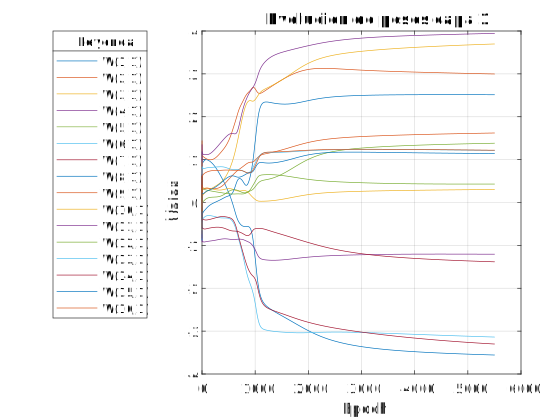
\includegraphics[width = 500pt, height = 500pt]{pol2/4}
	\caption{Gráfica 1.4}
\end{figure}

\begin{figure}[htpb]
	\centering
	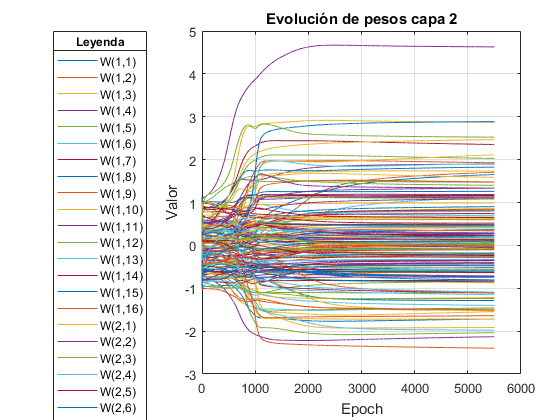
\includegraphics[width = 500pt, height = 500pt]{pol2/5}
	\caption{Gráfica 1.5}
\end{figure}

\begin{figure}[htpb]
	\centering
	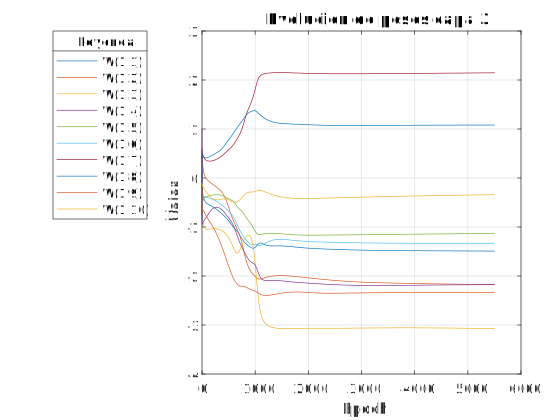
\includegraphics[width = 500pt, height = 500pt]{pol2/6}
	\caption{Gráfica 1.6}
\end{figure}

\begin{figure}[htpb]
	\centering
	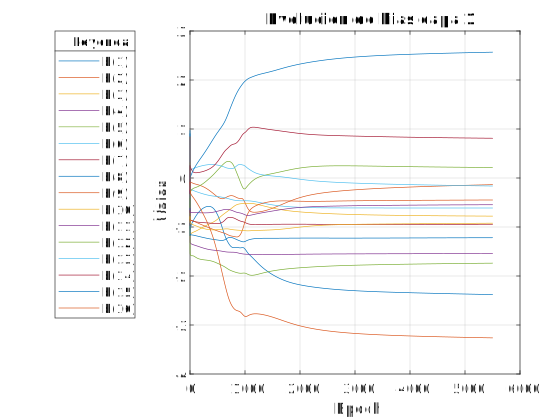
\includegraphics[width = 500pt, height = 500pt]{pol2/7}
	\caption{Gráfica 1.7}
\end{figure}

\begin{figure}[htpb]
	\centering
	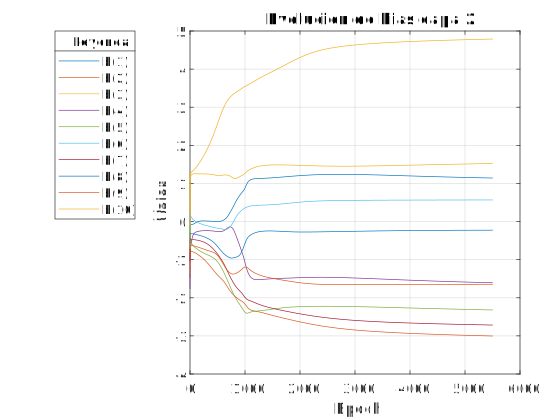
\includegraphics[width = 500pt, height = 500pt]{pol2/8}
	\caption{Gráfica 1.8}
\end{figure}

\begin{figure}[htpb]
	\centering
	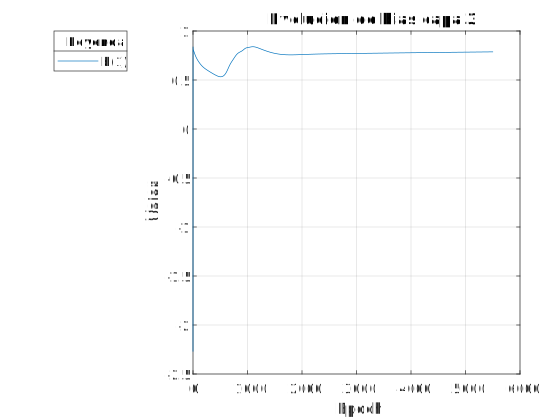
\includegraphics[width = 500pt, height = 500pt]{pol1/9}
	\caption{Gráfica 1.9}
\end{figure}
\newpage
\section{Discusión de Resultados}
Para cada uno de los resultados se muestra:
\begin{enumerate}
	\item Los datos con los cuales fue realizado el ejemplo.
	\item Los pesos y bias iniciales.
	\item La gráfica del ``historial'' de la evolución de los parámetros del perceptrón
	\item La gráfica de los vectores de entrada con su target y la frontera de desición final.
\end{enumerate}
\section{Conclusiones}
El perceptrón es la unidad básico de las redes neuronales que se usan hoy en día, su creador,  Frank Rosenblatt,  hizp una muy importante aportación para el campo de las redes neuronales artificiales. 
La práctica estuvo mucho más corta de lo que esperaba, la regla de aprendizaje es ``magia''. 
\section{Referencias}
Martin T Hagan. Machine Learning, Neural Network Design (2nd Edition), 2014.\\
\url{https://medium.com/@thomascountz/calculate-the-decision-boundary-of-a-single-perceptron-visualizing-linear-separability-c4d77099ef38}
\section{Apéndice}
\begin{lstlisting}[
style=Matlab-editor,
basicstyle=\mlttfamily,
escapechar=`,
caption={Código},
]
clc
clear

% Read the inputs file
inputs_path = strcat(input('Ingrese el nombre del archivo de inputs sin la extensión: ','s'), '.txt');
%inputs_path = 'inputs.txt';
inputs = importdata(inputs_path);

% Read the targets
targets_file = strcat(input('Ingrese el nombre del archivo de targets sin la extensión: ','s'), '.txt');
%targets_path = 'targets.txt';
targets = importdata(targets_path);

data_size = size(inputs, 1);

% Enter MLP architecture
architecture = str2num(input('Ingrese el vector de la arquitectura: ','s'));
% Calculate layer parameters
%architecture = str2num('1 16 10 1');
num_layers = length(architecture) - 1;
R = architecture(1);
functions_vector = str2num(input('Ingrese el vector de las funciones de activación: 1) purelin()\n2) logsig()\n3) tansig()\n\n: ','s'));
%functions_vector = str2num('3 2 1');

% Enter the learning factor
alpha = input('Ingresa el valor del factor de aprendizaje(alpha): ');
%alpha = .01;

epochmax = input('Ingresa el número máximo de épocas: ');
% epochmax = 10000;
%validation_iter = 500;
%numval = 7;
%error_epoch_validation = .0000000000000001;
numval = input('Numero maximo de incrementos consecutivos del error de validacion (numval): ');
error_epoch_validation = input('Ingrese el valor minimo del error de epoca (error_epoch_validation): ');
validation_iter = input('Ingrese el múltiplo de épocas para realizar una época de validación  (validation_iter): ');

% Dataset Slicing
config_option = input('Elija una configuración de distribución de datasets: \n1: 80-10-10\n2: 70-15-15\n');
%config_option = 2;
[training_ds, test_ds, validation_ds] = dataset_slices(config_option, inputs, targets);
validation_ds_size = size(validation_ds, 1);
test_ds_size = size(test_ds, 1);
training_ds_size = size(training_ds, 1);

disp('Dataset de entrenamiento:');
disp(training_ds);
disp('Dataset de validacion:');
disp(validation_ds);
disp('Dataset de prueba:');
disp(test_ds);

% Open the files for weights and bias
total_weight_files = 0;
total_bias_files = 0;
for i=1:num_layers
% For neurons
for j=1:architecture(i + 1)
% For weights
for l=1:architecture(i)
total_weight_files = total_weight_files + 1;
end
end
total_bias_files = total_bias_files + 1;
end

W_files = zeros(total_weight_files, 1);
b_files = zeros(total_bias_files, 1);

current_file = 1;
for i=1:num_layers
path = strcat(pwd, '/historico/capa_', num2str(i), '/pesos/');
if ~exist(path, 'dir')
mkdir(path);
end
% For layers
for j=1:architecture(i + 1)
% For neurons
for k=1:architecture(i)
archivo_pesos = strcat(path, '/pesos', num2str(j), '_', num2str(k),'.txt');
W_files(current_file) = fopen(archivo_pesos,'w');
current_file = current_file +1;
end
end
end

current_file = 1;
for i=1:num_layers
path = strcat(pwd,'/historico/capa_', num2str(i), '/bias/');
if ~exist(path, 'dir')
mkdir(path);
end
for j=1:architecture(i+1)
archivo_bias = strcat(path,'/bias',num2str(j),'.txt');
b_files(current_file) = fopen(archivo_bias,'w');
current_file = current_file +1;
end
end

% Initialize MLP parameters and Print them

num_w_files = 1;
num_b_files = 1;
W = cell(num_layers,1);
b = cell(num_layers,1);
% Output of each layer
a = cell(num_layers + 1, 1);
% Sentitivities
S = cell(num_layers, 1);
% Derivatives of each layer
F_m = cell(num_layers, 1);

% For each layer
for i=1:num_layers
% Random value
W_r_value = 2 * rand(architecture(i + 1), architecture(i)) - 1;
b_r_value = 2* rand(architecture(i + 1), 1) - i;
W{i} = W_r_value
b{i} = b_r_value
% For each neuron
for j=1:architecture(i + 1)
%For each weight
for k=1:architecture(i)
% Print wights value
fprintf(W_files(num_w_files), '%f\r\n', W_r_value(j, k));
num_w_files = num_w_files + 1;
end
end
% For each neuron
for j=1:architecture(i + 1)
% print bias value
fprintf(b_files(num_b_files), '%f\r\n', b_r_value(j));
num_b_files = num_b_files + 1;
end
end

% Learning algorithm
num_validation_epoch = 0;
early_stopping_increment = 0;
validation_error = 0;
learning_error = 0;
early_s_counter = 0;

% initialize vectors for printing errors
learning_err_values = zeros(epochmax, 1);
evaluation_err_values = zeros(ceil(epochmax / validation_iter), 1);
for epoch=1:epochmax
l_error = 0;
% Reset the values
num_w_files = 1;
num_b_files = 1;
% if isn't a validation epoch
if(mod(epoch ,validation_iter) ~= 0)
for t_data=1:training_ds_size    
% initial condition
a{1} = training_ds(t_data, 1); 
% Foward propagation
for t_p=1:num_layers
W_aux = cell2mat(W(t_p));
b_aux = cell2mat(b(t_p));
a_aux = cell2mat(a(t_p));
n_f = W_aux * a_aux + b_aux;
a{t_p + 1} = get_activation_function(n_f, functions_vector(t_p));
end
a_aux = cell2mat(a(num_layers + 1));
t_error = training_ds(t_data, 2) - a_aux;
l_error = l_error + (t_error / data_size);
% Sensitivities calculation
F_m{num_layers} = get_F_matrix(functions_vector(num_layers), architecture(num_layers + 1), a_aux);
F_m_temp = cell2mat(F_m(num_layers));
S{num_layers} = F_m_temp * (t_error)*(-2);
% Backpropagation
for m = num_layers-1:-1:1
W_aux = cell2mat(W(m+1));
s_aux = cell2mat(S(m+1));
a_aux = cell2mat(a(m+1));
F_m{m} = get_F_matrix(functions_vector(m),architecture(m+1),a_aux);
F_m_temp = cell2mat(F_m(m));
S{m} = F_m_temp * (W_aux')*s_aux;
end
% Learning Rules
for k = num_layers:-1:1
W_aux = cell2mat(W(k));
b_aux = cell2mat(b(k));
s_aux = cell2mat(S(k));
a_aux = cell2mat(a(k));
W{k} = W_aux - (alpha * s_aux * a_aux');
b{k} = b_aux - (alpha * s_aux);
W_aux = cell2mat(W(k));
b_aux = cell2mat(b(k));
end
end
learning_error = l_error;
learning_err_values(epoch) = l_error;      
% This epoch is a validation one
else
val_error = 0;
num_validation_epoch = num_validation_epoch + 1;
for t_data = 1:validation_ds_size
% Initial Condition
a{1} = validation_ds(t_data, 1);
% Foward propagation
for k=1:num_layers
W_aux = cell2mat(W(k));
a_aux = cell2mat(a(k));
b_aux = cell2mat(b(k));
n_f = W_aux * a_aux + b_aux;
a{k + 1} = get_activation_function(n_f, functions_vector(k));
end
a_aux = cell2mat(a(num_layers+1));
val_error = validation_ds(t_data,2)-a_aux;
val_error = val_error+(val_error/validation_ds_size);
end
evaluation_err_values(epoch) = val_error;
if early_stopping_increment == 0
validation_error = val_error;
early_stopping_increment = early_stopping_increment+1;
fprintf('Incremento actual para early stopping = %d\n', early_stopping_increment);
else
if val_error > validation_error
validation_error = val_error;
early_stopping_increment = early_stopping_increment+1;
fprintf('Incremento actual para early stopping = %d\n', early_stopping_increment);
if early_stopping_increment == numval
% Reset the counter
early_s_counter = 1;
fprintf('Early stopping en la época:  %d\n', epoch);
break;
end
else
validation_error = 0;
early_stopping_increment = 0;
fprintf('Incremento actual para early stopping = %d\n', early_stopping_increment);
end
end
end

% Print the values on console
num_w_files = 1;
num_b_files = 1;
for k = num_layers:-1:1
W_aux = cell2mat(W(k));
b_aux = cell2mat(b(k));
for j=1:architecture(k+1)
for l=1:architecture(k)
fprintf(W_files(num_w_files), '%f\r\n', W_aux(j,l));
num_w_files = num_w_files +1;
end
end
for j=1:architecture(k + 1)
fprintf(b_files(num_b_files), '%f\r\n', b_aux(j));
num_b_files = num_b_files + 1;
end
end

% Check stopping calculations
if mod(epoch,validation_iter) ~= 0 && l_error <= error_epoch_validation && l_error >= 0
learning_error = l_error;
fprintf('Aprendizaje exitoso en la época %d\n', epoch);
break;
end
end

if epoch == epochmax
disp('Se llego a epochmax');
end

% Print the las final values 
if early_s_counter == 1
num_w_files = 1;
num_b_files = 1;
for k = num_layers:-1:1
W_aux = cell2mat(W(k));
b_aux = cell2mat(b(k));
for j = 1:architecture(k + 1)
for l=1:architecture(k)
fprintf(W_files(num_w_files), '%f\r\n', W_aux(j, l));
num_w_files = num_w_files + 1;
end
end
for j=1:architecture(k + 1)
fprintf(b_files(num_b_files), '%f\r\n', b_aux(j));
num_b_files = num_b_files + 1;
end
end
end

% Close all files
for i=1:total_weight_files
fclose(W_files(i));
end
for i=1:total_bias_files
fclose(b_files(i));
end

% Propagate the test dataset
test_error = 0;
output = zeros(test_ds_size,1);
for i=1:test_ds_size
% Initial condition
a{1} = test_ds(i,1);
for k=1:num_layers
W_aux = cell2mat(W(k));
a_aux = cell2mat(a(k));
b_aux = cell2mat(b(k));
n_f = W_aux*a_aux+b_aux;
a{k+1} = get_activation_function(n_f, functions_vector(k));
end
test_data = cell2mat(a(1));
a_aux = cell2mat(a(num_layers + 1));
test_error = test_error + (1 / test_ds_size) * (test_ds(i,2) - a_aux);
output(i) = a_aux;
end

% Print last errors
fprintf('Error de aprendizaje = %f\n', learning_error);
fprintf('Error de validación = %f\n', validation_error);
fprintf('Error de prueba = %f\n', test_error);


% Output vs test
scatter_output_vs_test(test_ds, output);
% Propagate the training size for ploting

output = zeros(training_ds_size,1);
for i=1:training_ds_size
% Initial Condition
a{1} = training_ds(i, 1);
for k=1:num_layers
W_aux = cell2mat(W(k));
a_aux = cell2mat(a(k));
b_aux = cell2mat(b(k));
a{k+1} = get_activation_function(W_aux*a_aux+b_aux,functions_vector(k));
end
a_aux = cell2mat(a(num_layers + 1));
test_error = test_error + (1 / training_ds_size) * (training_ds(i,2) - a_aux);
output(i) = a_aux;
end

scatter_output_vs_training(training_ds, output);

% Plot the error evolution
error_plot(validation_iter, num_validation_epoch, learning_err_values, epoch, evaluation_err_values);
% Plot weight evolution
weight_evolution_plot(architecture, num_layers, epoch);
% Plot bias evolution
bias_evolution_plot(architecture, num_layers, epoch);

% Write final values
for i=1:num_layers
path = strcat(pwd, '/Valores_finales/capa_', num2str(i), '/');
if ~exist(path, 'dir')
mkdir(path);
end
W_aux = cell2mat(W(i));
res_pesos = strcat(path, '/pesos.txt');
dlmwrite(res_pesos, W_aux, ';');
end

for i=1:num_layers
path = strcat(pwd,'/Valores_finales/capa_', num2str(i), '/');
if ~exist(path, 'dir')
mkdir(path);
end
b_aux = cell2mat(b(i));
res_bias = strcat(path, '/bias.txt');
dlmwrite(res_bias, b_aux, ';');
end



\end{lstlisting}
\end{document}